\documentclass[dvipdfmx]{jsarticle}


\usepackage{tcolorbox}
\usepackage{color}
\usepackage{listings, plistings}

%% ノート/latexメモ
%% http://pepper.is.sci.toho-u.ac.jp/pepper/index.php?%A5%CE%A1%BC%A5%C8%2Flatex%A5%E1%A5%E2

%% JavaScriptの設定
%% https://e8l.hatenablog.com/entry/2015/11/29/232800
\lstdefinelanguage{javascript}{
  morekeywords = [1]{ %keywords
    await, break, case, catch, class, const, continue, debugger, default, delete, 
    do, else, enum, export, extends, finally, for, function, function*, if, implements, import, in, 
    instanceof, interface, let, new, package, private, protected, public, return, static, super,
    switch, this, throw, try, typeof, var, void, while, with, yield, yield*
  },
  morekeywords = [2]{ %literal
    false, Infinity, NaN, null, true, undefined
  },
  morekeywords = [3] { %Classes
    Array, ArrayBuffer, Boolean, DataView, Date, Error, EvalError, Float32Array, Float64Array,
    Function, Generator, GeneratorFunction, Int16Array, Int32Array, Int8Array, InternalError,
    JSON, Map, Math, Number, Object, Promise, Proxy, RangeError, ReferenceError, Reflect,
    RegExp, Set, String, Symbol, SyntaxError, TypeError, URIError, Uint16Array, Uint32Array,
    Uint8Array, Uint8ClampedArray, WeakMap, WeakSet
  },
  morecomment = [l]{//},
  morecomment = [s]{/*}{*/},
  morestring = [b]{"},
  morestring = [b]{'},
  alsodigit = {-},
  sensitive = true
}

%% 修正時刻: Tue 2022/03/15 10:04:41


% Java
\lstset{% 
  frame=single,
  backgroundcolor={\color[gray]{.9}},
  stringstyle={\ttfamily \color[rgb]{0,0,1}},
  commentstyle={\itshape \color[cmyk]{1,0,1,0}},
  identifierstyle={\ttfamily}, 
  keywordstyle={\ttfamily \color[cmyk]{0,1,0,0}},
  basicstyle={\ttfamily},
  breaklines=true,
  xleftmargin=0zw,
  xrightmargin=0zw,
  framerule=.2pt,
  columns=[l]{fullflexible},
  numbers=left,
  stepnumber=1,
  numberstyle={\scriptsize},
  numbersep=1em,
  language={Java},
  lineskip=-0.5zw,
  morecomment={[s][{\color[cmyk]{1,0,0,0}}]{/**}{*/}},
  keepspaces=true,         % 空白の連続をそのままで
  showstringspaces=false,  % 空白字をOFF
}
%\usepackage[dvipdfmx]{graphicx}
\usepackage{url}
\usepackage[dvipdfmx]{hyperref}
\usepackage{amsmath, amssymb}
\usepackage{itembkbx}
\usepackage{eclbkbox}	% required for `\breakbox' (yatex added)
\usepackage{enumerate}
\usepackage[default]{cantarell}
\usepackage[T1]{fontenc}
\fboxrule=0.5pt
\parindent=1em
\definecolor{mygrey}{rgb}{0.97, 0.97, 0.97}

\makeatletter
\def\verbatim@font{\normalfont
\let\do\do@noligs
\verbatim@nolig@list}
\makeatother

\begin{document}

%\anaumeと入力すると穴埋め解答欄が作れるようにしてる。\anaumesmallで小さめの穴埋めになる。
\newcounter{mycounter} % カウンターを作る
\setcounter{mycounter}{0} % カウンターを初期化
\newcommand{\anaume}[1][]{\refstepcounter{mycounter}{#1}{\boxed{\phantom{aa}\textnormal{\themycounter}\phantom{aa}}}} %穴埋め問題の空欄作ってる。
\newcommand{\anaumesmall}[1][]{\refstepcounter{mycounter}{#1}{\boxed{\tiny{\phantom{a}\themycounter \phantom{a}}}}}%小さい版作ってる。色々改造できる。

%% 修正時刻: Tue 2022/03/15 10:04:411


\section{2つのテーブルを結合する}

\subsection{内部結合(JOIN句)}

empテーブルの dept\_id は、deptテーブルの id である。

だから、dept\_idをキーにして、二つのテーブルを結合できる。

結合するには \textsf{JOIN}句を使う。

実行例

\begin{tcolorbox}
 mysql$>$ SELECT \ * \\
 \hspace{3mm} -$>$ FROM \ emp \\
 \hspace{3mm} -$>$ \underline{\textsf{INNER JOIN}} \ dept \\
 \hspace{3mm} -$>$ \underline{\textsf{ON}} \ emp.dept\_id \ = \ dept.id;
\end{tcolorbox}

\begin{lstlisting}[numbers=none, language=SQL]
 SELECT * 
 FROM メインの表
 [INNER] JOIN サブの表 
 ON メインの表.キーカラム名 = サブの表.キーカラム名
\end{lstlisting}


\vspace{3mm}
\begin{itemize}
 \item *(アスタリスク) --- メインの表、サブの表のすべての項目を表示する。
 \item emp.dept\_id --- emp表の dept\_id カラム名。ピリオドで区切って指定。
ピリオドの後に空白を入れてはいけない。
 \item dept.id --- dept表の id カラム名。
\end{itemize}


\vspace{3mm}
これで二つのテーブルが結合される。

% \begin{spacing}{0.8}        
% \begin{verbatim}
\begin{lstlisting}[numbers=none]
+----+------------+-----+----------+---------+-----+--------+
| id | name       | age | birthday | dept_id | id  | name   |
+----+------------+-----+----------+---------+-----+--------+
|  1 | 菅原文太    |  40 |     1933 | 001     | 001 | 総務部  |
|  2 | 千葉真一    |  34 |     1939 | 002     | 002 | 営業部  |
|  4 | 梶芽衣子    |  26 |     1947 | 002     | 002 | 営業部  |
|  3 | 北大路欣也  |  30 |     1943 | 003     | 003 | 経理部  |
+----+------------+-----+----------+---------+-----+--------+
\end{lstlisting}
% \end{verbatim}
% \end{spacing}

\textsf{JOIN} は \textsf{INNER JOIN} と記述できる。
``内部結合''と呼ばれている。

\textsf{ON emp.dept\_id = dept.id} は 
emp の dept\_id と dept の id が等しければ、そのレコードを抜き出す。

\rightline{※ emp.dept\_id は empテーブルの dept\_id という意味になる。}

\subsection{表示項目を絞る}

現在は項目を全て表示しているが、これを変更する。

emp表の id, name, age と dept表の name だけを表示させる。


\begin{lstlisting}[numbers=none, language=SQL]
 mysql> SELECT
     ->   emp.id,
     ->   emp.name,
     ->   age,
     ->   dept.name
     -> FROM emp
     -> INNER JOIN dept
     ->   ON emp.dept_id = dept.id;
\end{lstlisting}


% \begin{spacing}{0.8}        
% \begin{verbatim}
\begin{lstlisting}[numbers=none]
+----+------------+-----+--------+
| id | name       | age | name   |
+----+------------+-----+--------+
|  1 | 菅原文太   |  40 | 総務部 |
|  2 | 千葉真一   |  34 | 営業部 |
|  4 | 梶芽衣子   |  26 | 営業部 |
|  3 | 北大路欣也 |  30 | 経理部 |
+----+------------+-----+--------+
\end{lstlisting}
% \end{verbatim}
% \end{spacing}        

このように必要な項目のみ表示させることができる。
ただ、name という項目が二つあったり、英語であったりするので、
これを適切な日本語に変えることにする。

それには、\textsf{AS句} というのが使える。

たとえば、``emp.name AS 名前'' とすると、``emp.neme'' は ``名前'' と表示される。

\begin{lstlisting}[numbers=none, language=SQL]
 mysql> SELECT
     ->   emp.id AS ID,
     ->   emp.name AS 名前,
     ->   age AS 年齢,
     ->   dept.name AS 部署名
     -> FROM emp
     -> INNER JOIN dept
     ->   ON emp.dept_id = dept.id;
\end{lstlisting}


% \begin{spacing}{0.8}        
% \begin{verbatim}
\begin{lstlisting}[numbers=none]
+----+------------+------+--------+
| ID | 名前       | 年齢 | 部署名 |
+----+------------+------+--------+
|  1 | 菅原文太   |   40 | 総務部 |
|  2 | 千葉真一   |   34 | 営業部 |
|  4 | 梶芽衣子   |   26 | 営業部 |
|  3 | 北大路欣也 |   30 | 経理部 |
+----+------------+------+--------+
\end{lstlisting}
% \end{verbatim}
% \end{spacing}

さらによく見てみると、この表は部署名の順に並んでいる。
これを ID順に並びかえる。

そのためには \textsf{ORDER句} というのが使える。

たとえば、今回の場合だと、\fbox{\textsf{ORDER BY emp.id [\! ASC\! ]}} とすることで、ID順になる。

\textsf{ASC} というのは''昇順''という意味で、省略すると ASC と指定したことになる。

また、\textsf{DESC} と指定すると ''降順'' で並びかえできる。


\begin{lstlisting}[numbers=none, language=SQL]
 mysql> SELECT
     ->   emp.id AS ID,
     ->   emp.name AS 名前,
     ->   age AS 年齢,
     ->   dept.name AS 部署名
     -> FROM emp
     -> INNER JOIN dept
     ->   ON emp.dept_id = dept.id
     -> ORDER BY ID;
\end{lstlisting}



\begin{lstlisting}[numbers=none]
+----+------------+------+--------+
| ID | 名前       | 年齢 | 部署名 |
+----+------------+------+--------+
|  1 | 菅原文太   |   40 | 総務部 |
|  2 | 千葉真一   |   34 | 営業部 |
|  3 | 北大路欣也 |   30 | 経理部 |
|  4 | 梶芽衣子   |   26 | 営業部 |
+----+------------+------+--------+
\end{lstlisting}


\textsf{ORDER BY emp.id} とするところを \textsf{ORDER BY ID} としている。

これは、1行目で \textsf{emp.id AS ID} としているので、ID を使うことができるのである。


\subsection{テーブルの指定を簡略化する}

emp とか dept とかのテーブルの指定も別名を使うことで簡略化できる。

\begin{lstlisting}[numbers=none, language=SQL]
 mysql> SELECT
     ->   e.id AS ID,
     ->   e.name AS 名前,
     ->   age AS 年齢,
     ->   d.name AS 部署名
     -> FROM emp AS e
     -> INNER JOIN dept AS d
     ->   ON e.dept_id = d.id
     -> ORDER BY ID;
\end{lstlisting}


さらに、FROM や JOIN の後では、すぐ後ろに 別名(ここでは e や d のこと)がくる場合、{\em AS} は
省略できる。

\begin{lstlisting}[numbers=none, language=SQL]
 mysql> SELECT
     ->   e.id AS ID,
     ->   e.name AS 名前,
     ->   age AS 年齢,
     ->   d.name AS 部署名
     -> FROM emp e
     -> INNER JOIN dept d
     ->   ON e.dept_id = d.id
     -> ORDER BY ID;
\end{lstlisting}







\newpage
\subsection{外部結合(LEFT OUTER JOIN / RIGHT OUTER JOIN)}

\subsubsection{左外部結合 LEFT OUTER JOIN}

この emp表に次のデータを追加する。

\begin{tcolorbox}
 \begin{tabular}{lcl}
  ID & : & 5 \\
  名前 & : & 成田三樹夫 \\
  年齢 & : &  38 \\
  誕生年 & : & 1935 \\
  部署ID & : & (なし) \\
 \end{tabular}
\end{tcolorbox}

\begin{lstlisting}[numbers=none, language=SQL]
 mysql> INSERT INTO emp
     ->   (name, age, birthday)
     -> VALUES
     ->   ('成田三樹夫', 38, 1935);
\end{lstlisting}


\begin{spacing}{0.8}        
\begin{verbatim}
mysql> SELECT * FROM emp;
+----+------------+-----+----------+---------+
| id | name       | age | birthday | dept_id |
+----+------------+-----+----------+---------+
|  1 | 菅原文太   |  40 |     1933 | 001     |
|  2 | 千葉真一   |  34 |     1939 | 002     |
|  3 | 北大路欣也 |  30 |     1943 | 003     |
|  4 | 梶芽衣子   |  26 |     1947 | 002     |
|  5 | 成田三樹夫 |  38 |     1935 | NULL    |
+----+------------+-----+----------+---------+    
\end{verbatim}
\end{spacing}


このデータには dept\_id、つまり部署ID がない。たとえば社長とかの場合である。

この状態で 内部結合 をすると、どうなるか?

\begin{verbatim}
mysql> SELECT
    ->   e.id AS ID,
    ->   e.name AS 名前,
    ->   e.age AS 年齢,
    ->   d.name AS 部署名
    -> FROM emp e
    -> JOIN dept d
    ->   ON e.dept_id = d.id
    -> ORDER BY ID;
\end{verbatim}

\begin{spacing}{0.8}        
\begin{verbatim}
+----+------------+------+--------+
| ID | 名前       | 年齢 | 部署名 |
+----+------------+------+--------+
|  1 | 菅原文太   |   40 | 総務部 |
|  2 | 千葉真一   |   34 | 営業部 |
|  3 | 北大路欣也 |   30 | 経理部 |
|  4 | 梶芽衣子   |   26 | 営業部 |
+----+------------+------+--------+    
\end{verbatim}
\end{spacing}

結合表には出てこない。

これを図であらわすと、このようになる。

\vspace{3mm}
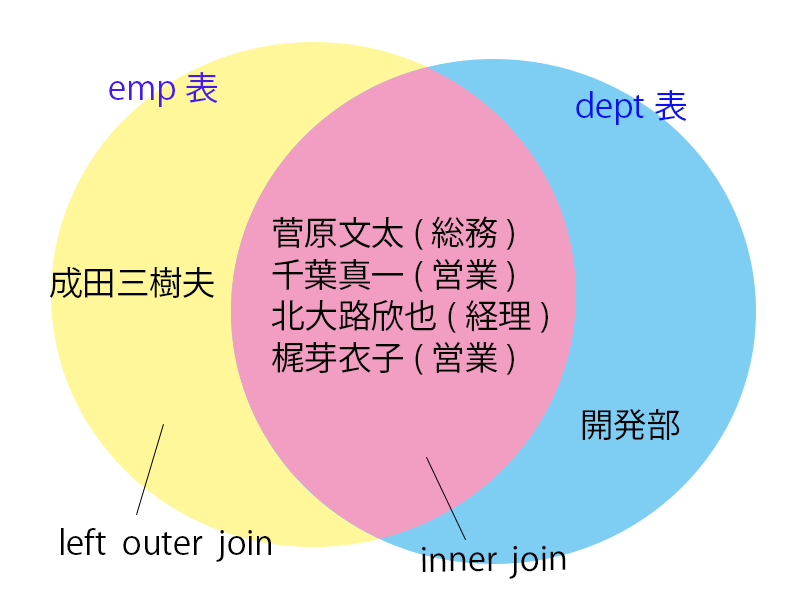
\includegraphics[width=13cm]{../06-mysql/ketsugo.png}
\vspace{3mm}

成田三樹夫は部署IDがないので結合の対象ではない。

こんなときは \emph{左外部結合(LEFT [OUTER] JOIN)} を使う。

\begin{lstlisting}[numbers=none, language=SQL]
 mysql> SELECT
     ->   e.id AS ID,
     ->   e.name AS 名前,
     ->   e.age AS 年齢,
     ->   d.name as 部署名
     -> FROM emp e
     -> LEFT OUTER JOIN dept d
     ->   ON e.dept_id = d.id
     -> ORDER BY ID;
\end{lstlisting}

\rightline{※ LEFT JOIN と記述することもできる}

\begin{spacing}{0.8}        
\begin{verbatim}
+----+------------+------+--------+
| ID | 名前       | 年齢 | 部署名 |
+----+------------+------+--------+
|  1 | 菅原文太   |   40 | 総務部 |
|  2 | 千葉真一   |   34 | 営業部 |
|  3 | 北大路欣也 |   30 | 経理部 |
|  4 | 梶芽衣子   |   26 | 営業部 |
|  6 | 成田三樹夫 |   38 | NULL   |
+----+------------+------+--------+
\end{verbatim}
\end{spacing}

\subsubsection{右外部結合 RIGHT [OUTER] JOIN}

また、dept表をみてみると、\textsf{id : '004'} が  \textsf{開発部} であるが、
emp表には dept\_id が '004' である人はいない。

この状態で結合表をつくり、開発部という項目も表示させるには、次のようにする。

\begin{lstlisting}[numbers=none, language=SQL]
 mysql> SELECT
     ->   e.id AS ID,
     ->   e.name AS 名前,
     ->   e.age AS 年齢,
     ->   d.name AS 部署名
     -> FROM emp e
     -> RIGHT OUTER JOIN dept d
     ->   ON e.dept_id = d.id
     -> ORDER BY ID;
\end{lstlisting}

\begin{spacing}{0.8}        
\begin{verbatim}
+------+------------+------+--------+
| ID   | 名前       | 年齢 | 部署名 |
+------+------------+------+--------+
| NULL | NULL       | NULL | 開発部 |
|    1 | 菅原文太   |   40 | 総務部 |
|    2 | 千葉真一   |   34 | 営業部 |
|    3 | 北大路欣也 |   30 | 経理部 |
|    4 | 梶芽衣子   |   26 | 営業部 |
+------+------------+------+--------+
\end{verbatim}
\end{spacing}

\newpage
\section{練習問題}

\subsection{結合の練習}

\fbox{4.2 テーブル作成問題(2)} で作った4つの表を結合しましょう。

gender表、state表、course表、person表 を内部結合して、以下のように表示させてください。

\vspace{3mm}
\begin{tabular}{|c|l|c|l|l|l|} \hline
 ID & 名前            & 性別   & 誕生日     & 出身         & コース            \\ \hline\hline 
  1 & 染谷将太        & 男     & 1992-09-03 & 東京都       & JavaScriptコース  \\ \hline
  3 & 渡辺哲          & 男     & 1950-03-11 & 愛知県       & Javaコース        \\ \hline
  4 & 窪塚洋介        & 男     & 1979-05-07 & 神奈川県     & HTML/CSSコース    \\ \hline
  2 & 二階堂ふみ      & 女     & 1994-09-21 & 沖縄県       & PHPコース         \\ \hline
  5 & 吉高由里子      & 女     & 1988-07-22 & 東京都       & Javaコース        \\ \hline
\end{tabular}
\vspace{3mm}

\begin{lstlisting}[numbers=none, language=SQL]
mysql> SELECT
    ->   timestampdiff(YEAR, birthday, curdate()) AS 年齢
    -> FROM person;
\end{lstlisting}

とすると、以下のように出力できる。

\vspace{3mm}
\begin{tabular}{|c|} \hline
 年齢 \\ \hline\hline
  29  \\ \hline
  27  \\ \hline
  71  \\ \hline
  42  \\ \hline
  33  \\ \hline
\end{tabular}
\vspace{3mm}

このことから、以下のように表示させることができるはず。

\vspace{3mm}
\begin{tabular}{|c|l|c|l|l|l|} \hline
 ID & 名前            & 性別   & 年齢 & 出身         & コース            \\ \hline\hline 
  1 & 染谷将太        & 男     & 29  & 東京都       & JavaScriptコース  \\ \hline
  3 & 渡辺哲          & 男     & 71  & 愛知県       & Javaコース        \\ \hline
  4 & 窪塚洋介        & 男     & 42  & 神奈川県     & HTML/CSSコース    \\ \hline
  2 & 二階堂ふみ      & 女     & 27  & 沖縄県       & PHPコース         \\ \hline
  5 & 吉高由里子      & 女     & 33  & 東京都       & Javaコース        \\ \hline
\end{tabular}
\vspace{3mm}




\end{document}

%% 修正時刻: Sat May  2 15:10:04 2020


%% 修正時刻: Sun 2022/10/02 05:17:442
